\section{Initial Greedy Algorithm}
\label[section]{sec:failedalg}
\begin{leftbar}
    \noindent
    \textbf{Motivation:} 
    Since time coherence only exists as a connection from one set of streamlines to another, we started by creating an algorithm capable of generating such streamlines.
    We could then use this algorithm to generate sets of streamlines for time frames without time coherence as a negative example and to illustrate the effects of its absence.
    Initially, the algorithm was developed for the 2D case, the extension to 3D is shown in subsection 4.1.2.
\end{leftbar}
\noindent
The algorithm uses two operations, streamline traversal and seed filtering,
which are executed round-robin until there is no more room for new streamlines.
The result of the algorithm is a space-filling set of streamlines with even spacing in 3D fields.\\
We use 2 essential parameters to control how the images are generated.
The first one, $d_s$, is the neighbor search distance. 
It controls the distance from the current streamline where new streamlines start at,
allowing us to fill the whole space.
In order to add longer liens while guaranteeing even spacing,
we introduce a second parameter $d_c$, which is the neighbor cutoff distance.
As soon as a streamline comes within this distance to another streamline, it is terminated.\\
The typical range for $d_c$ is $0.5\,d_s \leq d_c \leq 0.75\,d_s$.
Making $d_c$ smaller than $0.5\,d_s$ allows streamlines to get very close,
introducing visual clutter and a crowded appearance.
At values $\geq0.75\,d_s$, a lot of streamlines are very short in forward or backward time due to the proximity of $d_s$ and $d_c$,
causing most of them to be removed immediately.

\newpage
\subsection{Two-Dimensional Implementation}
\begin{figure}[ht]
    \centering
    \begin{subfigure}[b]{0.3\textwidth}
        \centering
        \begin{tikzpicture}[domain=0:4, scale=.8]
    \draw[very thin,color=gray] (-0.1,-0.1) grid (3.9,3.9);

    \draw[->] (-0.2,0) -- (4.2,0) node[right] {$x$};
    \draw[->] (0,-0.2) -- (0,4.2) node[above] {$y$};

    \draw[dotted, thick]                       (1.5,0) -- (1.5,1) -- (1.73,1.87) -- (2.3,2.78) -- (3,3.4) -- (4,4);
    \draw plot[only marks, mark=x] coordinates{(1.5,0)               (1.73,1.87)    (2.3,2.78)    (3,3.4)};
    
    \draw[red] plot[only marks, mark=*] coordinates{      (1.5,1)};
\end{tikzpicture}

        \caption*{(a)}
    \end{subfigure}
    \begin{subfigure}[b]{0.3\textwidth}
        \centering
        \begin{tikzpicture}[domain=0:4, scale=.8]
    \draw[very thin,color=gray] (-0.1,-0.1) grid (3.9,3.9);
    
    \draw[->] (-0.2,0) -- (4.2,0) node[right] {$x$};
    \draw[->] (0,-0.2) -- (0,4.2) node[above] {$y$};
    
    \draw[dotted, thick]                       (1.5,0) -- (1.5,1) -- (1.73,1.87) -- (2.3,2.78) -- (3,3.4) -- (4,4);
    \draw plot[only marks, mark=x] coordinates{(1.5,0)               (1.73,1.87)    (2.3,2.78)    (3,3.4)};
    
    \draw[black ,arrows={Circle[green]-Circle[green]}] (0.6,  1.1 ) -- (2.4 , 0.9 );
    \draw[black ,arrows={Circle[green]-Circle[green]}] (0.91, 2.2 ) -- (2.59, 1.53);
    \draw[black ,arrows={Circle[green]-Circle[green]}] (1.57, 3.33) -- (3.05, 2.2 );
    \draw[black ,arrows={Circle[green]-Circle[green]}] (2.5 , 4   ) -- (3.55, 2.75);

    \draw[red] plot[only marks, mark=*] coordinates{(1.5,1)};
\end{tikzpicture}

        \caption*{(b)}
    \end{subfigure}
    \begin{subfigure}[b]{0.3\textwidth}
        \centering
        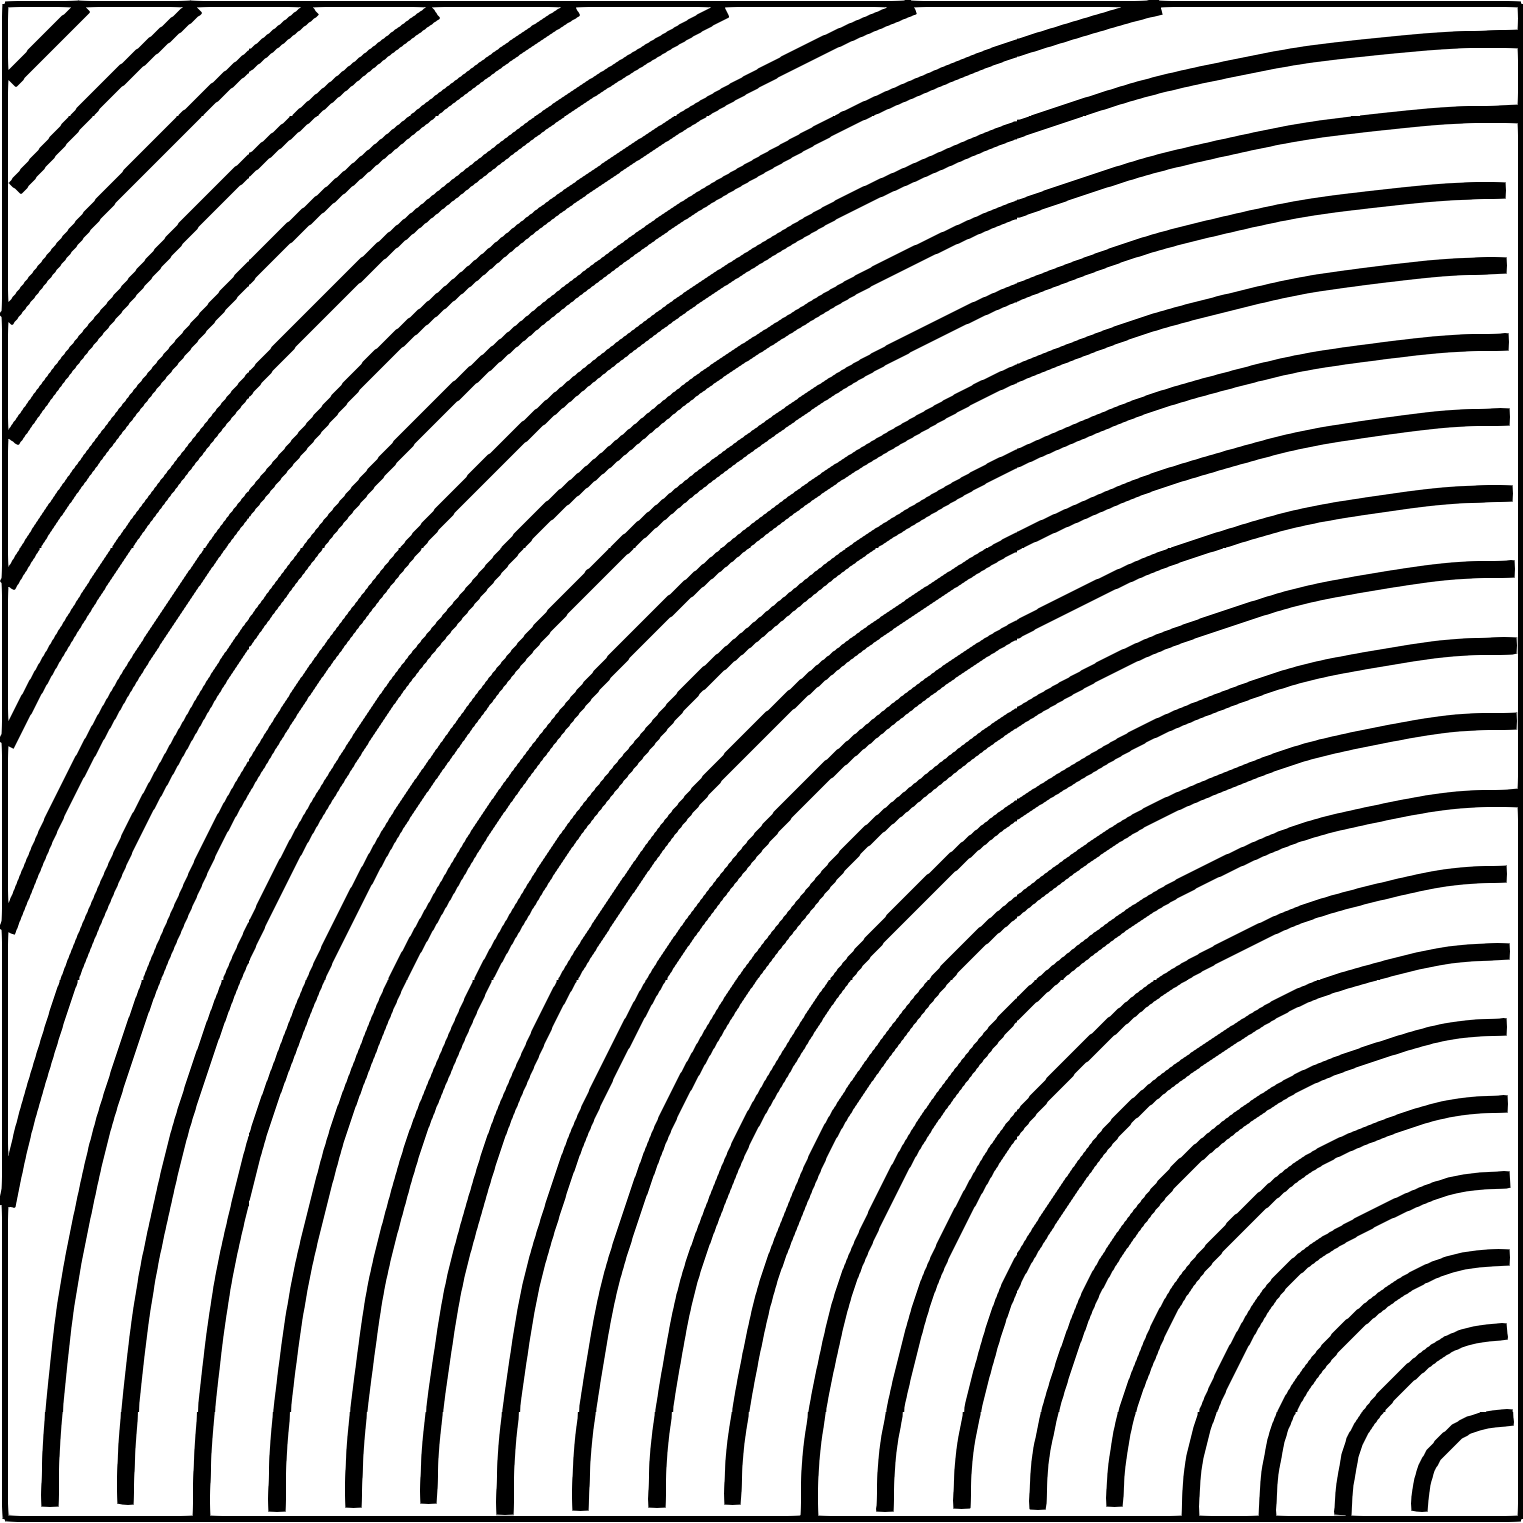
\includegraphics[scale=.1]{figures/OldAlgRotate.png}
        \caption*{(c)}
    \end{subfigure}
    \caption{
        (a): Forward and backward streamline integration through the field starting at the seed (red).
        The chosen sample points are drawn as a cross, and include the seed.
        (b): Equidistant seed candidates (green) obtained from the normals at the sample points are chosen for the next iteration.
        (c): Lines with equal distance generated by our algorithm in a field defined by $u(x,y)=(y, -x)$.}
    \label[figure]{fig:failedbasics}
\end{figure}
\vspace{-1cm}
\subsubsection{Streamline Traversal}
First, we choose a seed point from a list of candidates (initially an arbitrary point from the dataset) and remove it from the list.
Then we integrate forward and backward (\cref{fig:failedbasics} (a)) to obtain the other points on the streamline,
until a number of steps is reached, we cross the bounding box, or we get too close to another streamline.
If the total length of the streamline is too small, we remove it.\\
To obtain the seed candidates, we compute the normals of the field at these points, and add points a distance $d_s$ away from them to the list (\cref{fig:failedbasics} (b)).
\subsubsection{Seed Filtering}
The number of neighbor seed candidates is roughly 2$n$, where $n$ is the number of samples of the streamline we are integrating.
To quickly remove seeds that cannot produce a good streamline, we use two filtering conditions.
The first condition arises from the fact that roughly half the seeds generated by a streamline $L_1$ during the traversal process will lie close to - if not exactly on - the preceding streamline, $L_0$.
This happens because the seeds are placed a distance $d_s$ away, 
while the streamlines are mostly that same distance apart themselves.
The second condition is the distance to other seeds,
as starting a streamline from a seed that is too close to another will immediately end it.
Therefore, we filter two sets of seeds: The ones generated during the traversal process and those present in the entire field.
\begin{figure}[ht]
    \centering
    \begin{subfigure}[b]{0.4\textwidth}
        \centering
        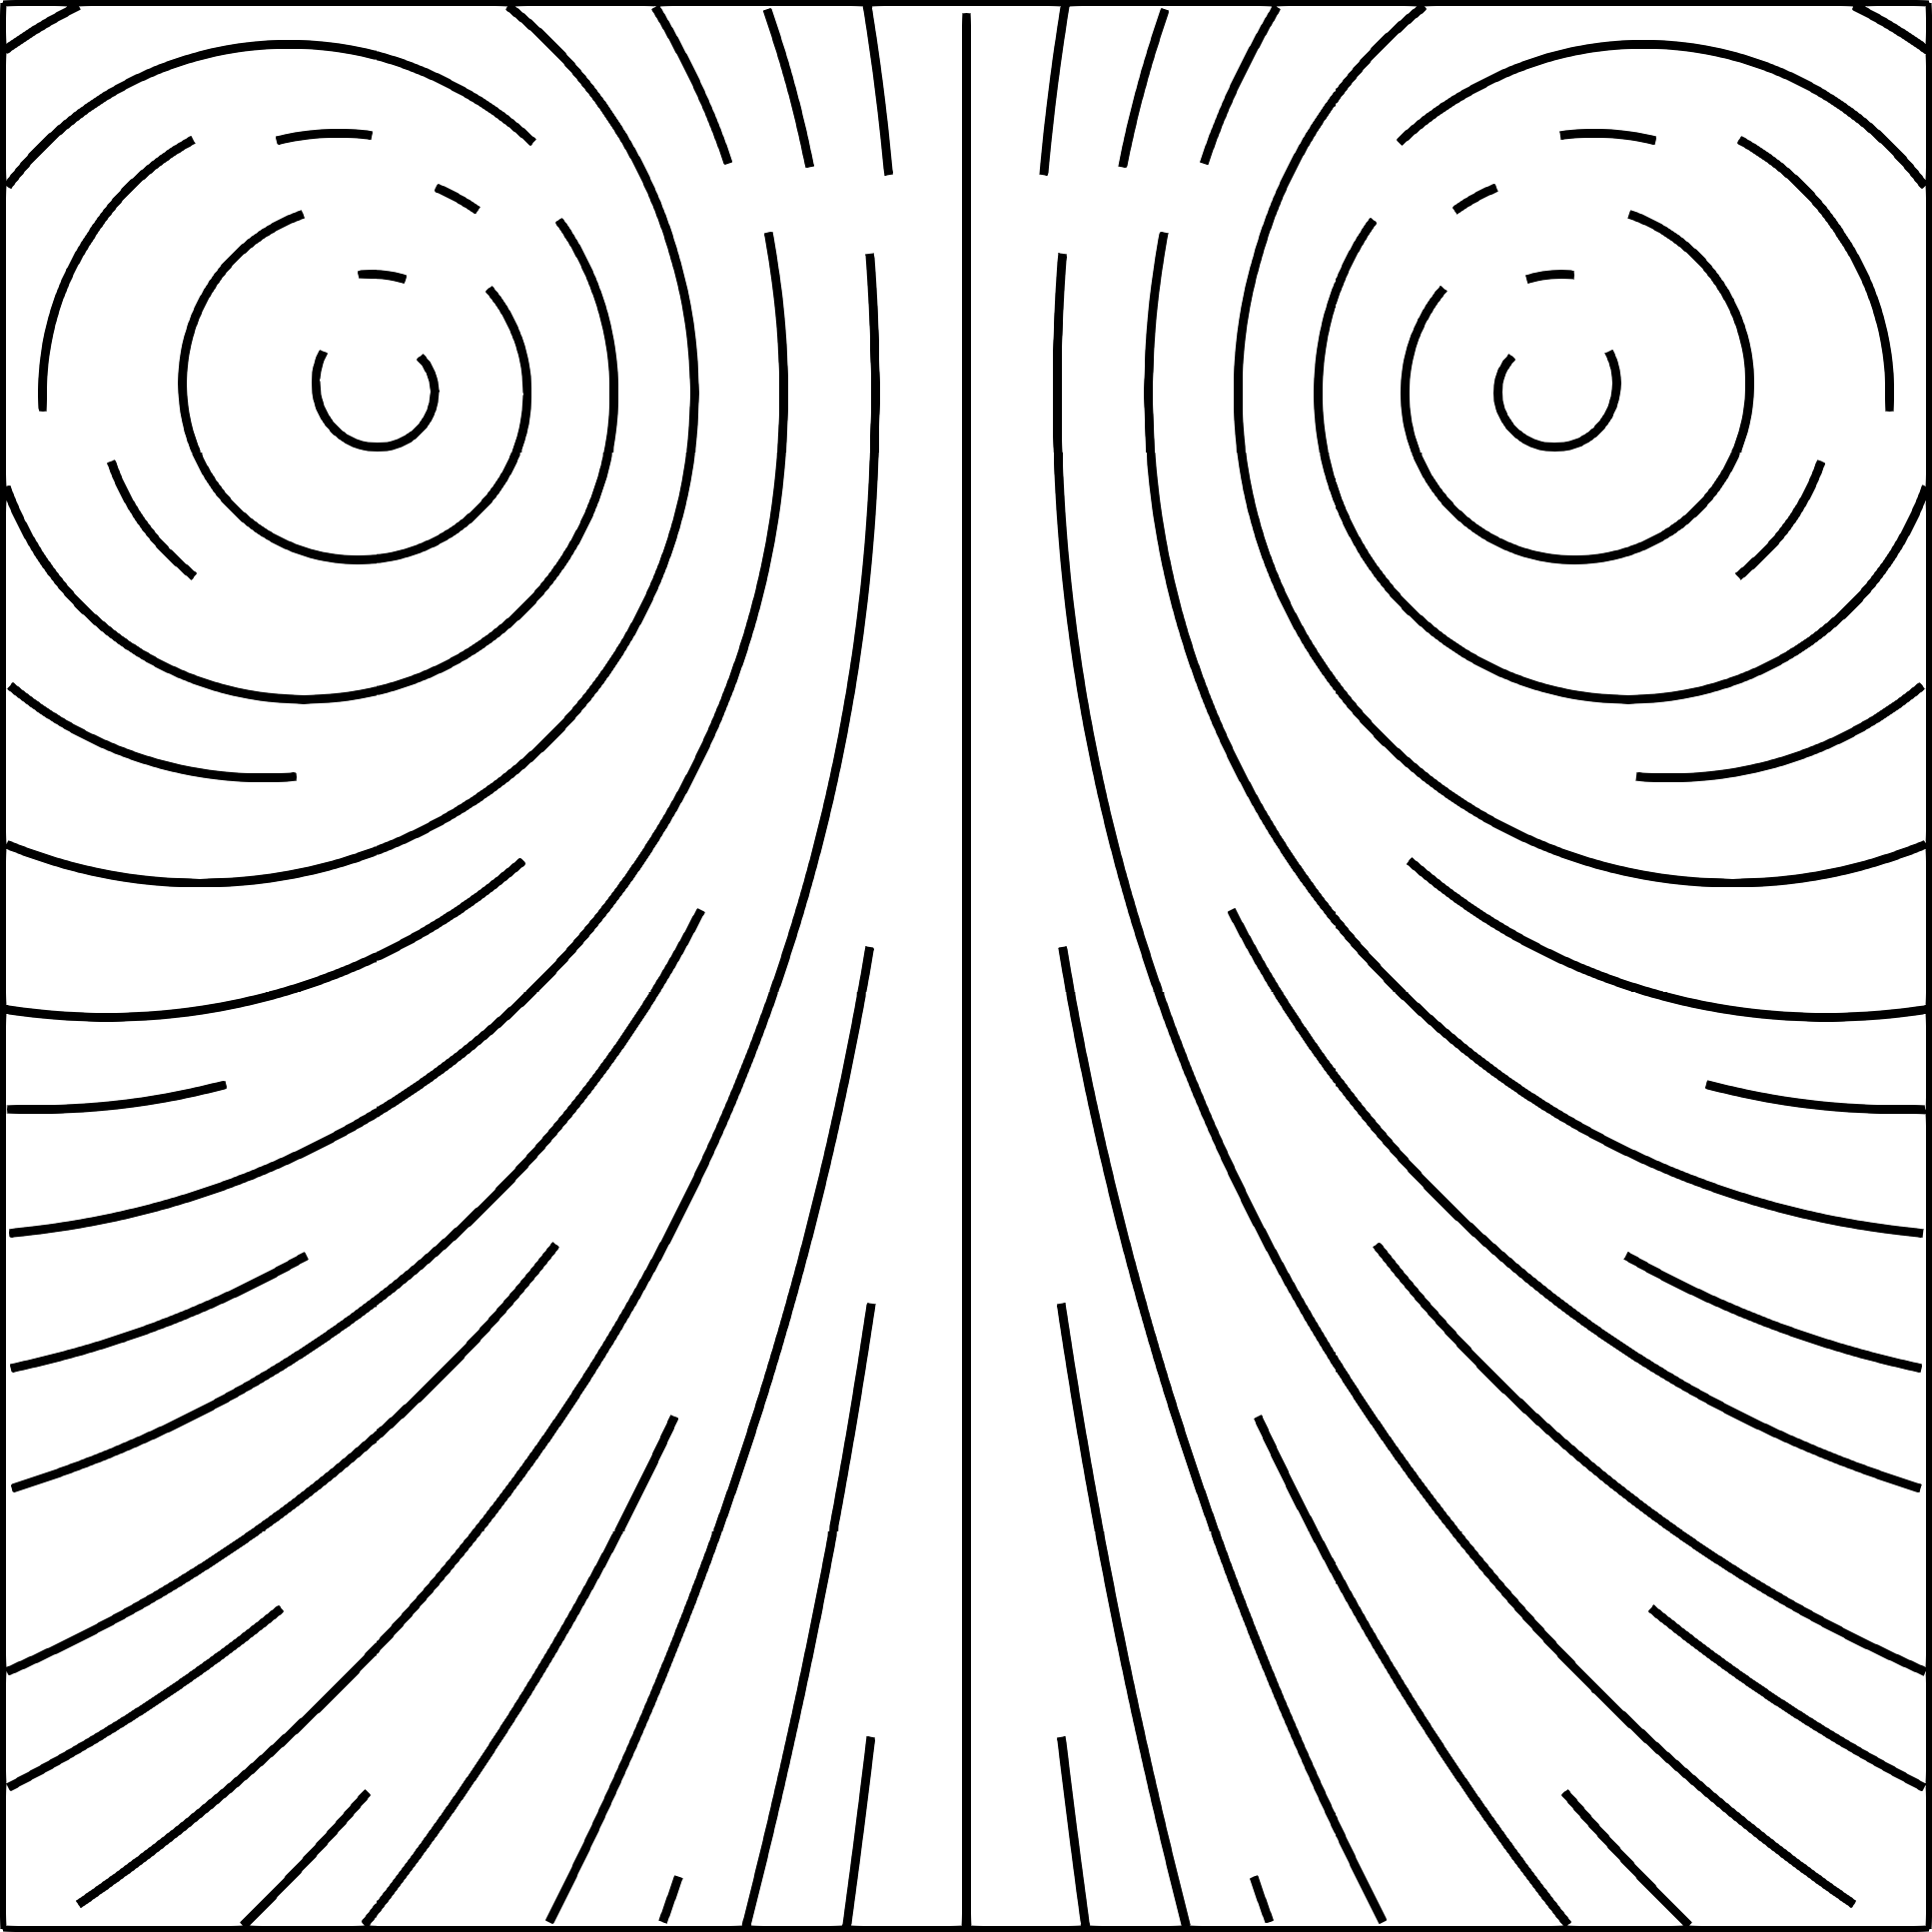
\includegraphics[scale=.1]{figures/OldAlgOrbit.png}
        \caption*{(a)}
    \end{subfigure}
    \begin{subfigure}[b]{0.4\textwidth}
        \centering
        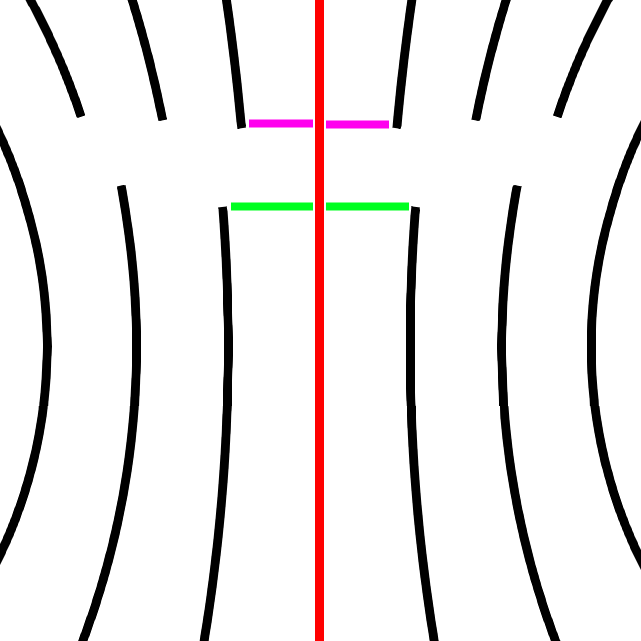
\includegraphics[scale=.3]{figures/OldAlgOrbitDistsZoom.png}
        \caption*{(b)}
    \end{subfigure}
    \caption{
        (a): The streamlines created in a double gyro dataset.
        (b): Top center view of (a). New streamlines created from the center streamline (red) are cut off due to reaching $d_c$ (magenta). New streamlines are only drawn at distance grater than $d_c$, producing the gap between the upper and lower three streamlines (black).
        The lower streamlines continue at a distance of $d_S$ (green).
    }
\end{figure}
\subsubsection{Line Cutoff and Optimization}
In order to quickly filter the $2n$-pairs for points on the parent streamline, we store the parent's points and remove any of the $2n$ seeds from the current step if they are too close.
When removing other seeds we come across, we employ a grid with a spacing of $d_c$ and use a dictionary to obtain lists of points inside the grid cell.
If we add a point during integration, we simply look up the coordinate and its 8 neighboring cells as a key to points in the area.
If a seed closer than $d_c$ is found in those cells, it is subsequently removed.
This allows for an easy way to end the integration when getting too close to another streamline as well:
We need only keep track of whether we came close to another streamline's points during integration
(provided the integration step size is less than $d_c$, which is usually the case).

\newpage
\subsection{Steady Field Streamline Placement in 3D}
\label[section]{sec:3D}
% The most important part to generate streamlines in 3D is obtaining the seed locations.
% In three dimensions, a vector has infinitely many normals, which all lie on a plane it is a normal of.
% Therefore, we define a number of points to evenly distribute around the streamline.
% The process of obtaining these points is as follows.
% \rule[2mm]{\textwidth}{0.4pt}
% \begin{minipage}{.6\textwidth}
%     Instead of the two trivial normals in 2D, we now construct a normal plane around the streamline trajectory at the streamline's points.
%     For this, we find two vectors which are linearly independent of each other and the trajectory, and then use NumPy's QR-decomposition to orthonormalize them.
%     The algorithm returns three orthonormalized column vectors, the first of which has a direction equal to the first provided input vector.
%     We can therefore feed it the streamline segment's direction and two basis vectors, and receive two orthonormal basis vectors $b_0, b_1$.
% \end{minipage}
% \begin{minipage}{.39\textwidth}
%     \centering
%     \setlength\pgfplotswidth{1.2\textwidth}
%     \begin{tikzpicture}
    \begin{axis}[ 
        ticks=none,
        axis lines = middle,
        axis line style={->},
        ymin=-.6, ymax=2.1,
        xmin=-.6, xmax=2.1,
        xlabel={$x$},
        ylabel={$z$},
        width=\pgfplotswidth,
        height=\pgfplotswidth
        ]
        \draw[rotate around={45:(.5,1)}] (axis cs:.5,1) ellipse (.6 and 1) [radius=1, fill=white];
        % Segment
        \draw[rotate around={45:(.5,1)}, ->, dotted, thick, red] (.5, 1) -- (1.5, 1) node[right] {$s$};
        % b0, b1
        \draw[rotate around={45:(.5,1)}, ->, blue!50] (.5, 1) -- (-.05, .85) node[right] {$b_0$};
        \draw[rotate around={45:(.5,1)}, ->, blue!50] (.5, 1) -- (.68, .09) node[right] {$b_1$};
      
        \draw[->] (0, 0) -- (-.5, -.5) node[right] {$y$};
    \end{axis}
\end{tikzpicture}

% \end{minipage}
% \rule{\textwidth}{0pt}
% \rule[3mm]{\textwidth}{0.4pt}
% \begin{minipage}{.6\textwidth}
%     Having found $b_0$ and $b_1$, we can use the roots of unity to find evenly spaced points on the unit circle.
%     With $i$ being the complex number, we obtain $k$ roots of unity via 
%     \vspace{-2mm}
%     \[n_j = e^{ji2\pi/k}, j = 0, 1, ..., k-1\]
%     \vspace{-2mm}
%     Since the magnitude of $n_j$ is always one, we do a simple basis transformation into the 3D frame of reference.
%     We obtain the $j$-th 3D-vector $v_j$ from the $j$-th root using our basis vectors $b_0$ and $b_1$:
%     \vspace{-2mm}
%     \[v_j = re(n_j)*b_0 + im(n_j)*b_1 \]
% \end{minipage}
% \begin{minipage}{.39\textwidth}
%     \centering
%     \setlength\pgfplotswidth{1.2\textwidth}
%     \begin{tikzpicture}
    \tikzset{
        pics/carc/.style args={#1:#2:#3}{
            code={
               \draw[pic actions] (#1:#3) arc(#1:#2:#3);
            }
        }
    }
    \begin{axis}[ 
        ticks=none,
        axis lines = middle,
        axis line style={->},
        ymin=-1.3, ymax=1.3,
        xmin=-1.3, xmax=1.3,
        xlabel={$1$},
        ylabel={$i$},
        width=\pgfplotswidth,
        height=\pgfplotswidth
        ]
        \draw (0,0) circle [radius=1, fill=white];
        \draw[very thick] (0,0) pic[red]{carc=0:72:2cm};
        \node[red] at (1,1) {$\frac{2\pi}{5}$};

        \draw[very thick, ->] (0,0) -- (1,0) node[midway, above right] {$n_0$};
        \draw[very thick, ->] (0,0) -- ( .309, .951) node[midway, right] {$n_1$};
        \draw[very thick, ->] (0,0) -- (-.809, .588) node[midway, above] {$n_2$};
        \draw[very thick, ->] (0,0) -- (-.809,-.588) node[midway, below] {$n_3$};
        \draw[very thick, ->] (0,0) -- ( .309,-.951) node[midway, right] {$n_4$};
    \end{axis}
\end{tikzpicture}

% \end{minipage}
% \rule[-1mm]{\textwidth}{0.4pt}
% This gives us $k$ uniformly placed vectors in the normal plane around the current streamline segment.
% The rest of the algorithm stays largely the same as in 2D, the grid used for seed filtering is extended into the 3rd dimension accordingly.
% See figure 4.5 on the next page for an example using a 3D vector field.
% \newpage
% \begin{figure}[ht]
%     \centering
%     \begin{subfigure}[b]{0.5\textwidth}
%         \centering
%         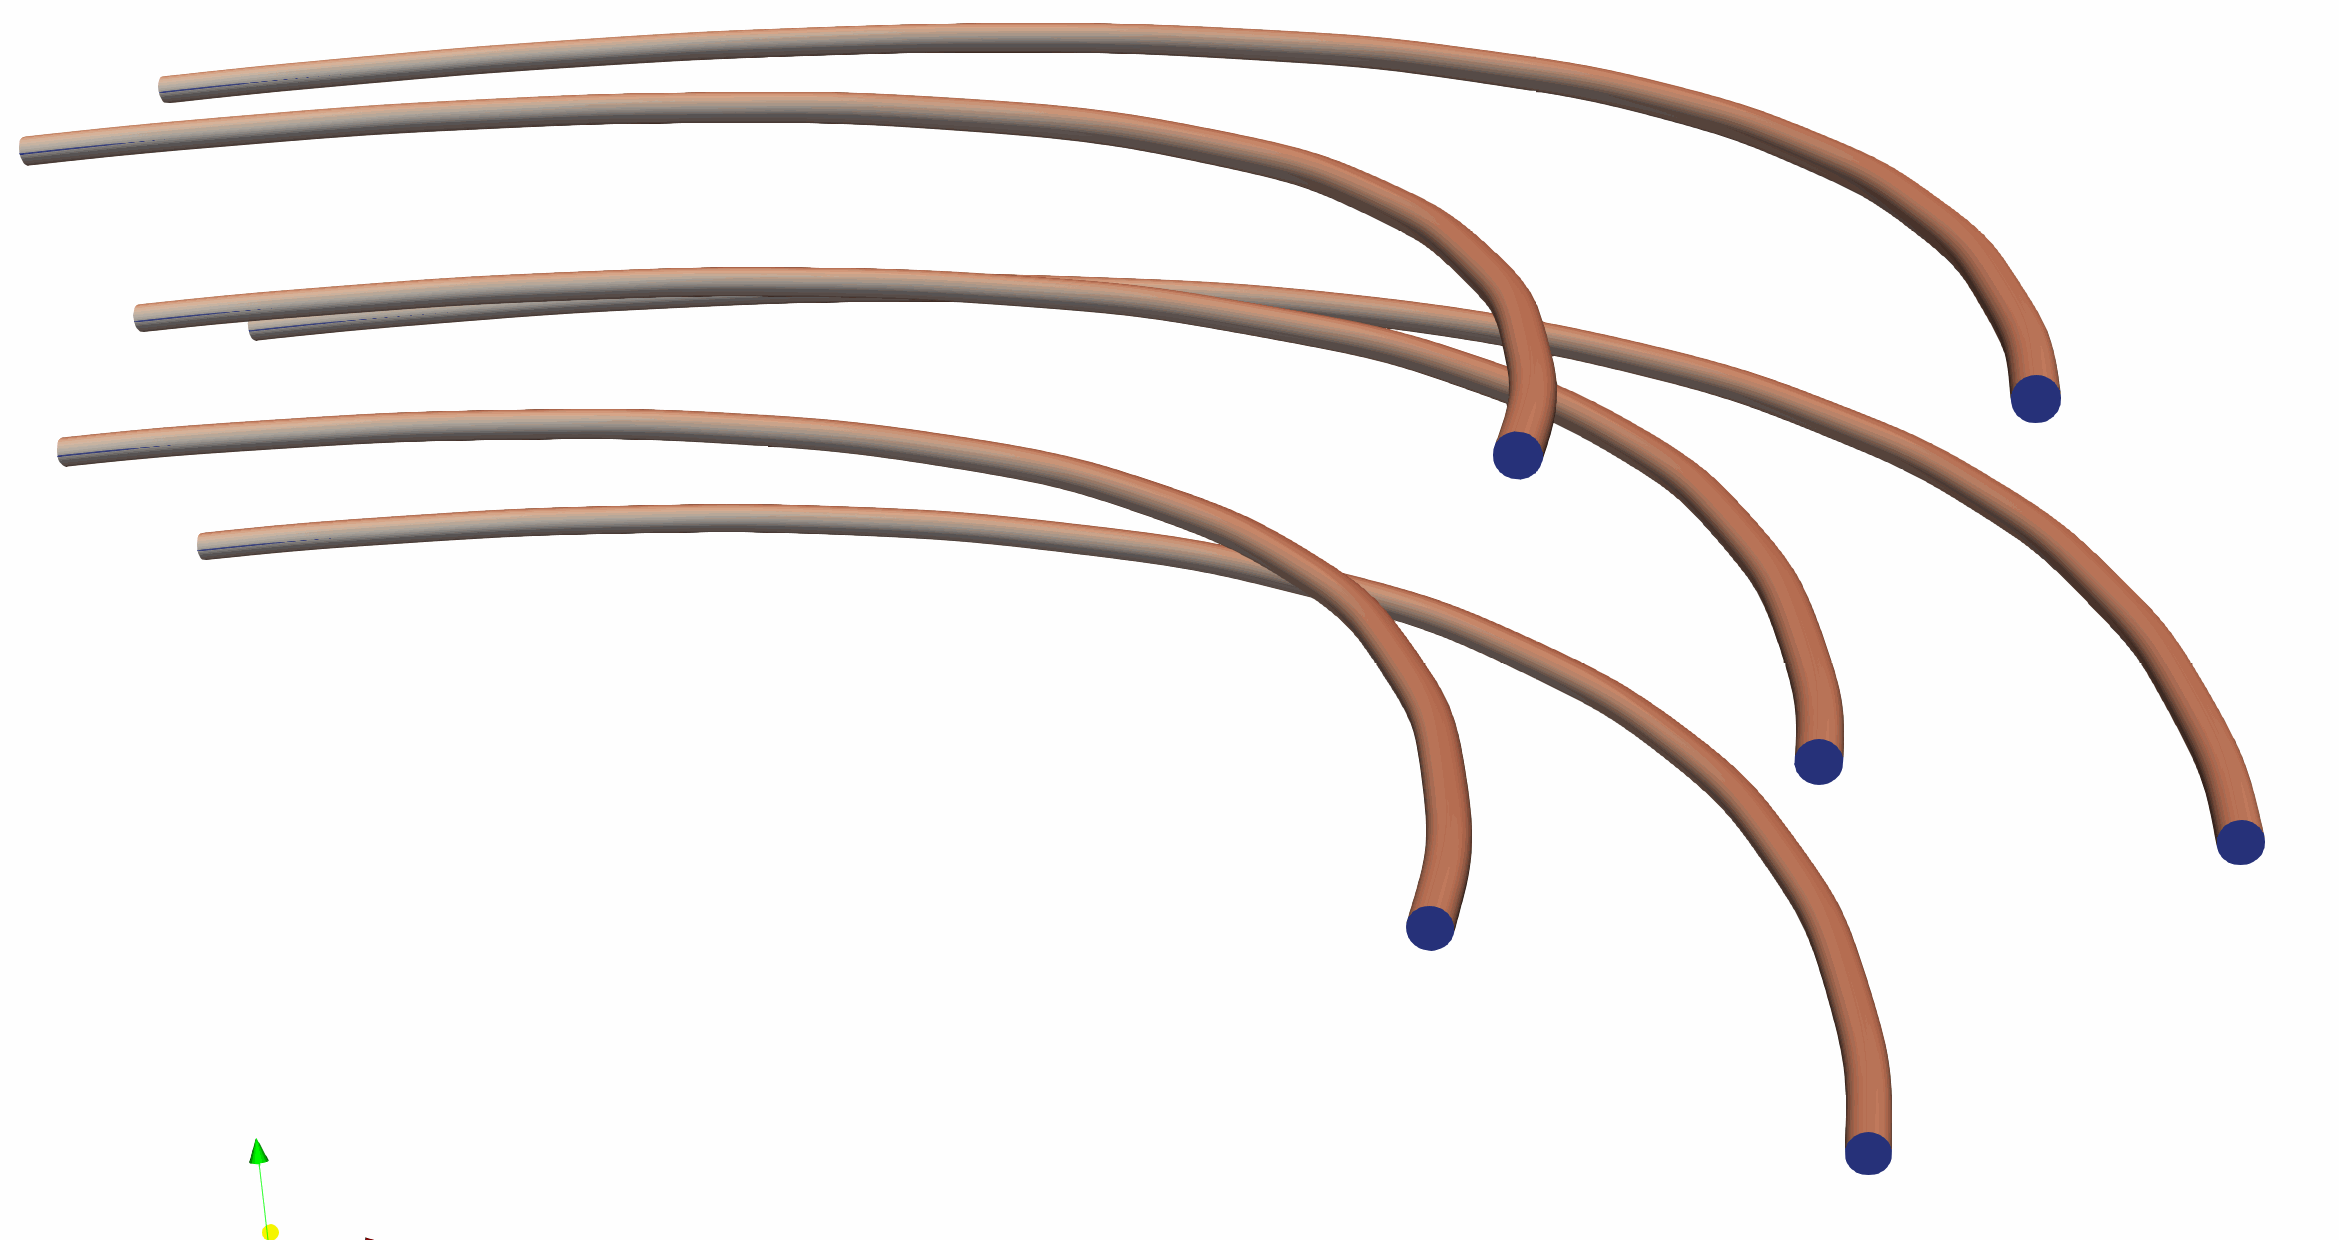
\includegraphics[scale=.1]{figures/OldAlg3D5.png}
%         \caption*{(a)}
%     \end{subfigure}
%     \begin{subfigure}[b]{0.4\textwidth}
%         \centering
%         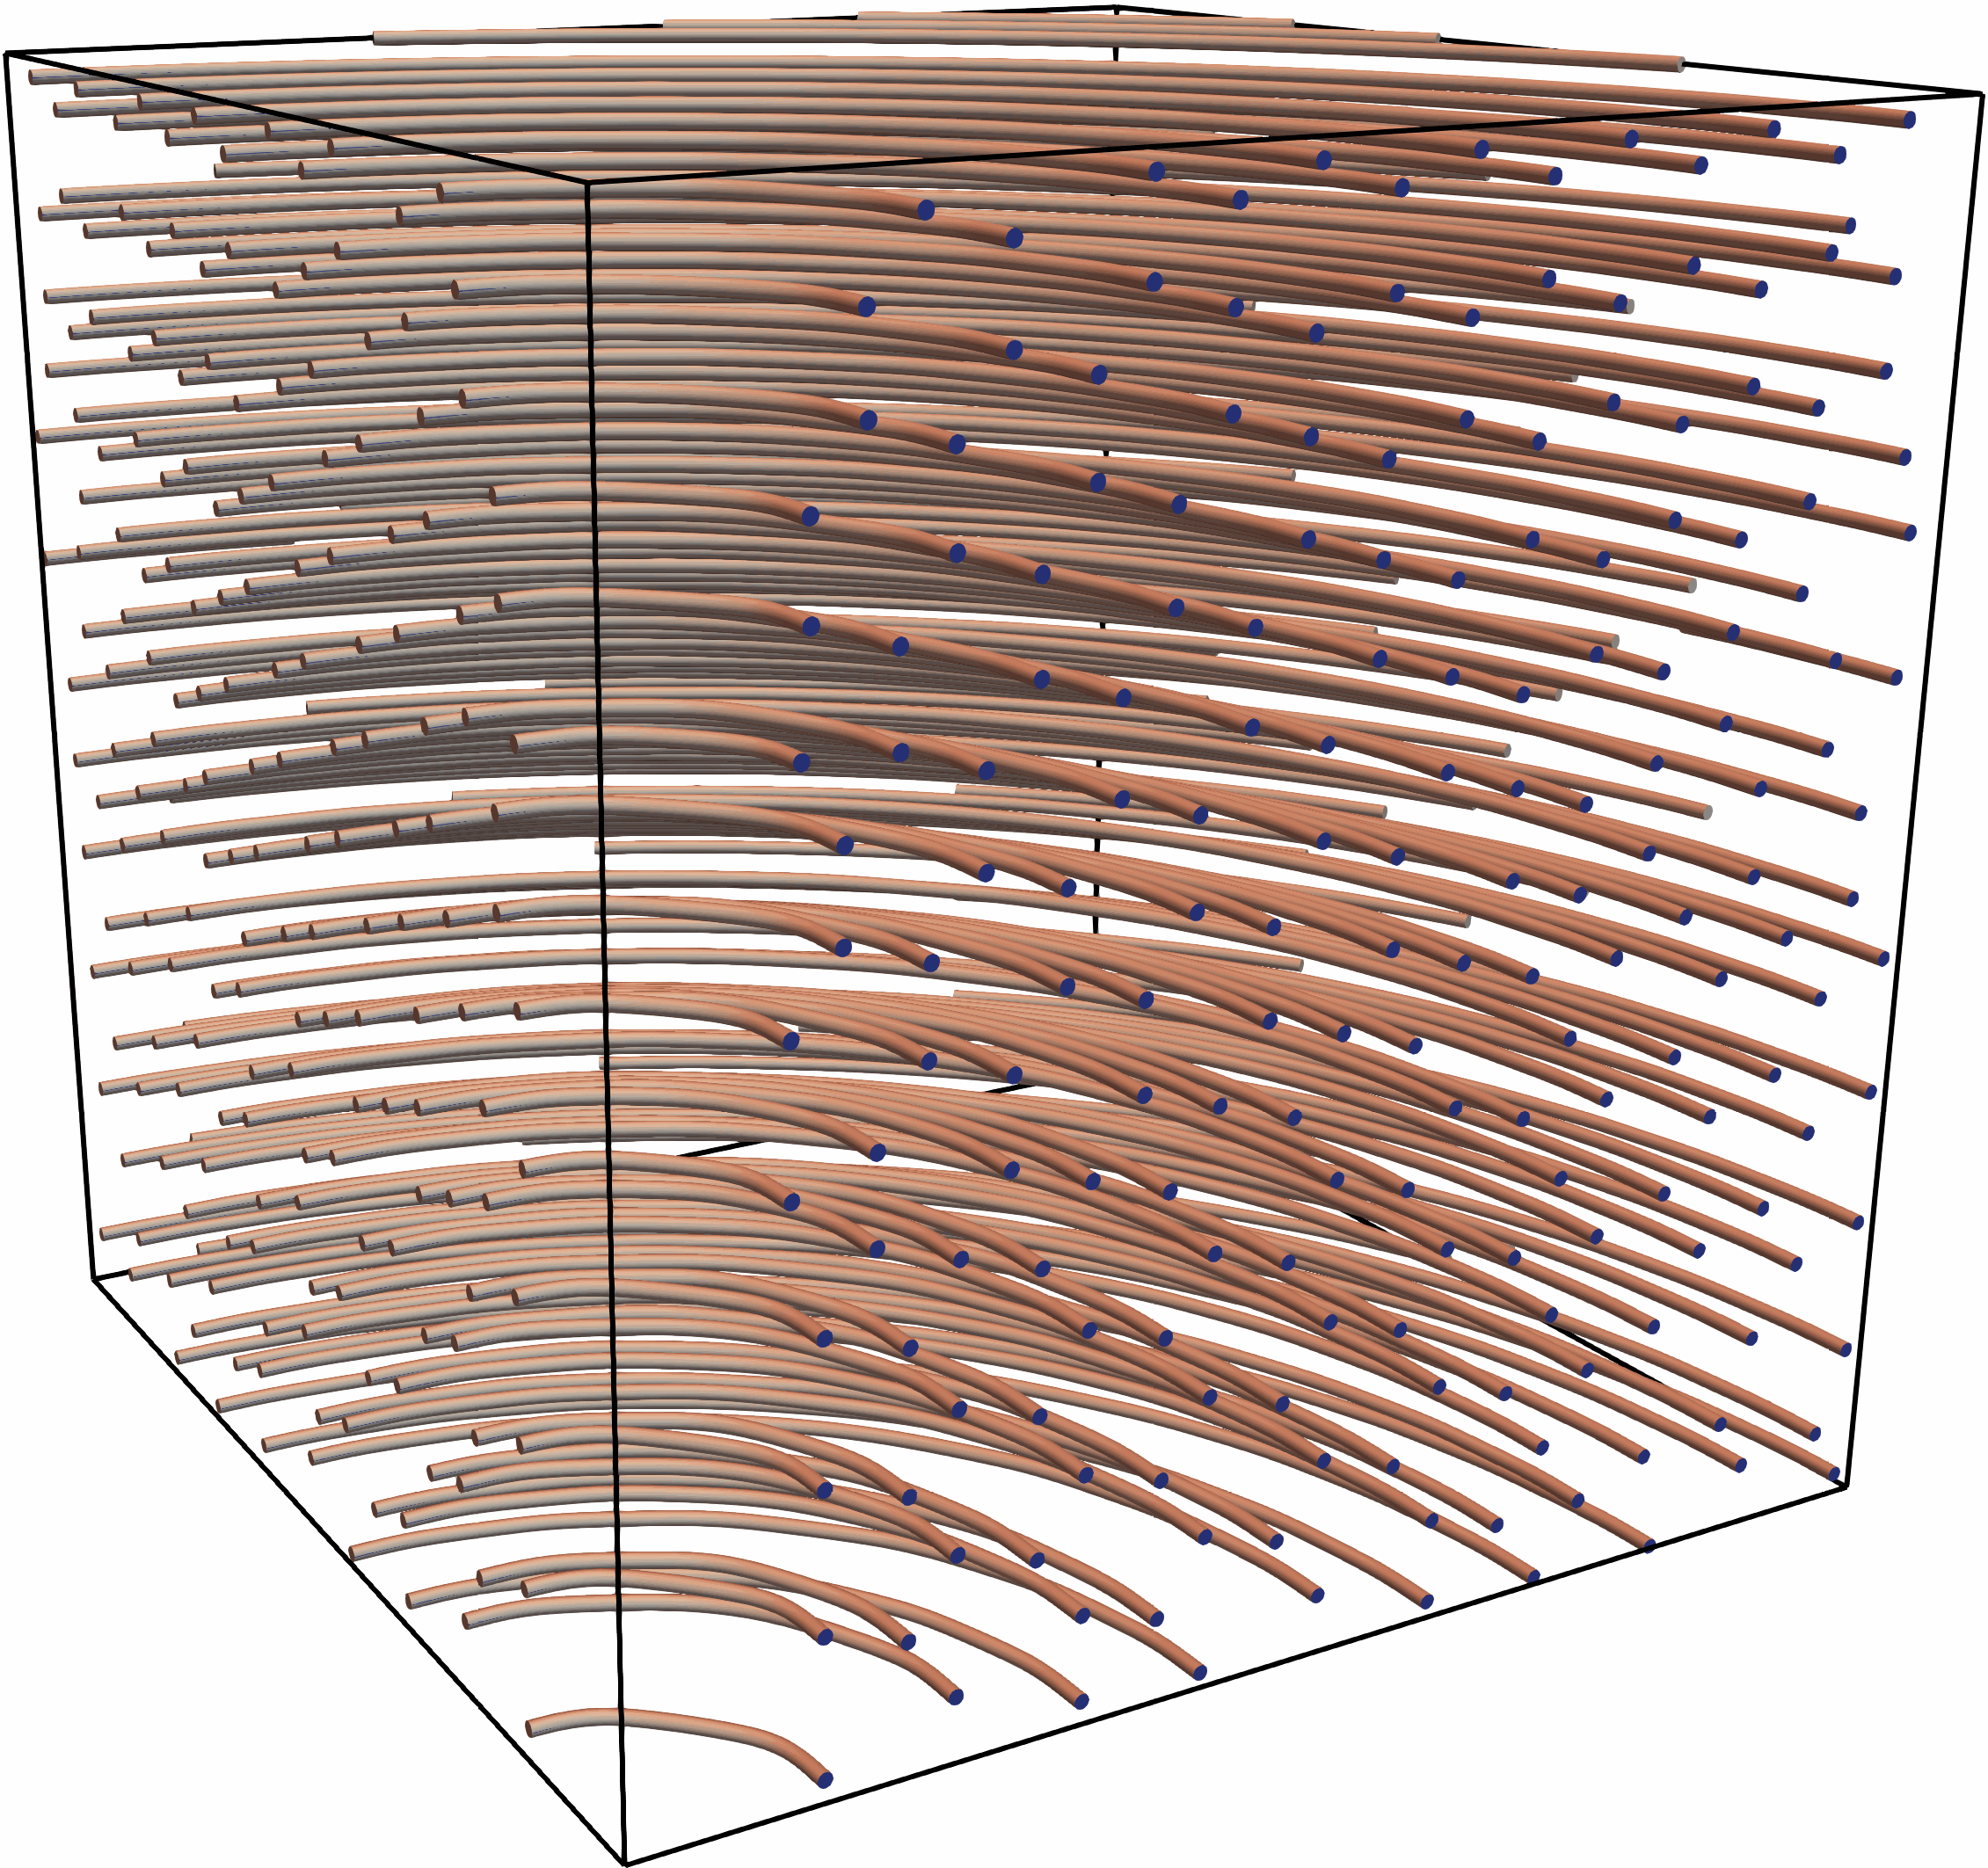
\includegraphics[scale=.09]{figures/OldAlg3D400.png}
%         \caption*{(b)}
%     \end{subfigure}
%     \caption{
%         (a): A clear view of the center streamline with five neighbor streamlines evenly distributed at distance $d_S$.
%         (b): A filled cube containing 254 streamlines. Notice the resemblance to Figure 4.1 (c).
%     }
% \end{figure}
\begin{figure}[ht]
    \centering
    \begin{subfigure}{.33\textwidth}
        \centering
        \setlength\pgfplotswidth{\textwidth}
        \begin{tikzpicture}
    \begin{axis}[ 
        ticks=none,
        axis lines = middle,
        axis line style={->},
        ymin=-.6, ymax=2.1,
        xmin=-.6, xmax=2.1,
        xlabel={$x$},
        ylabel={$z$},
        width=\pgfplotswidth,
        height=\pgfplotswidth
        ]
        \draw[rotate around={45:(.5,1)}] (axis cs:.5,1) ellipse (.6 and 1) [radius=1, fill=white];
        % Segment
        \draw[rotate around={45:(.5,1)}, ->, dotted, thick, red] (.5, 1) -- (1.5, 1) node[right] {$s$};
        % b0, b1
        \draw[rotate around={45:(.5,1)}, ->, blue!50] (.5, 1) -- (-.05, .85) node[right] {$b_0$};
        \draw[rotate around={45:(.5,1)}, ->, blue!50] (.5, 1) -- (.68, .09) node[right] {$b_1$};
      
        \draw[->] (0, 0) -- (-.5, -.5) node[right] {$y$};
    \end{axis}
\end{tikzpicture}

        \caption*{(a)}
    \end{subfigure}
    \begin{subfigure}{.33\textwidth}
        \centering
        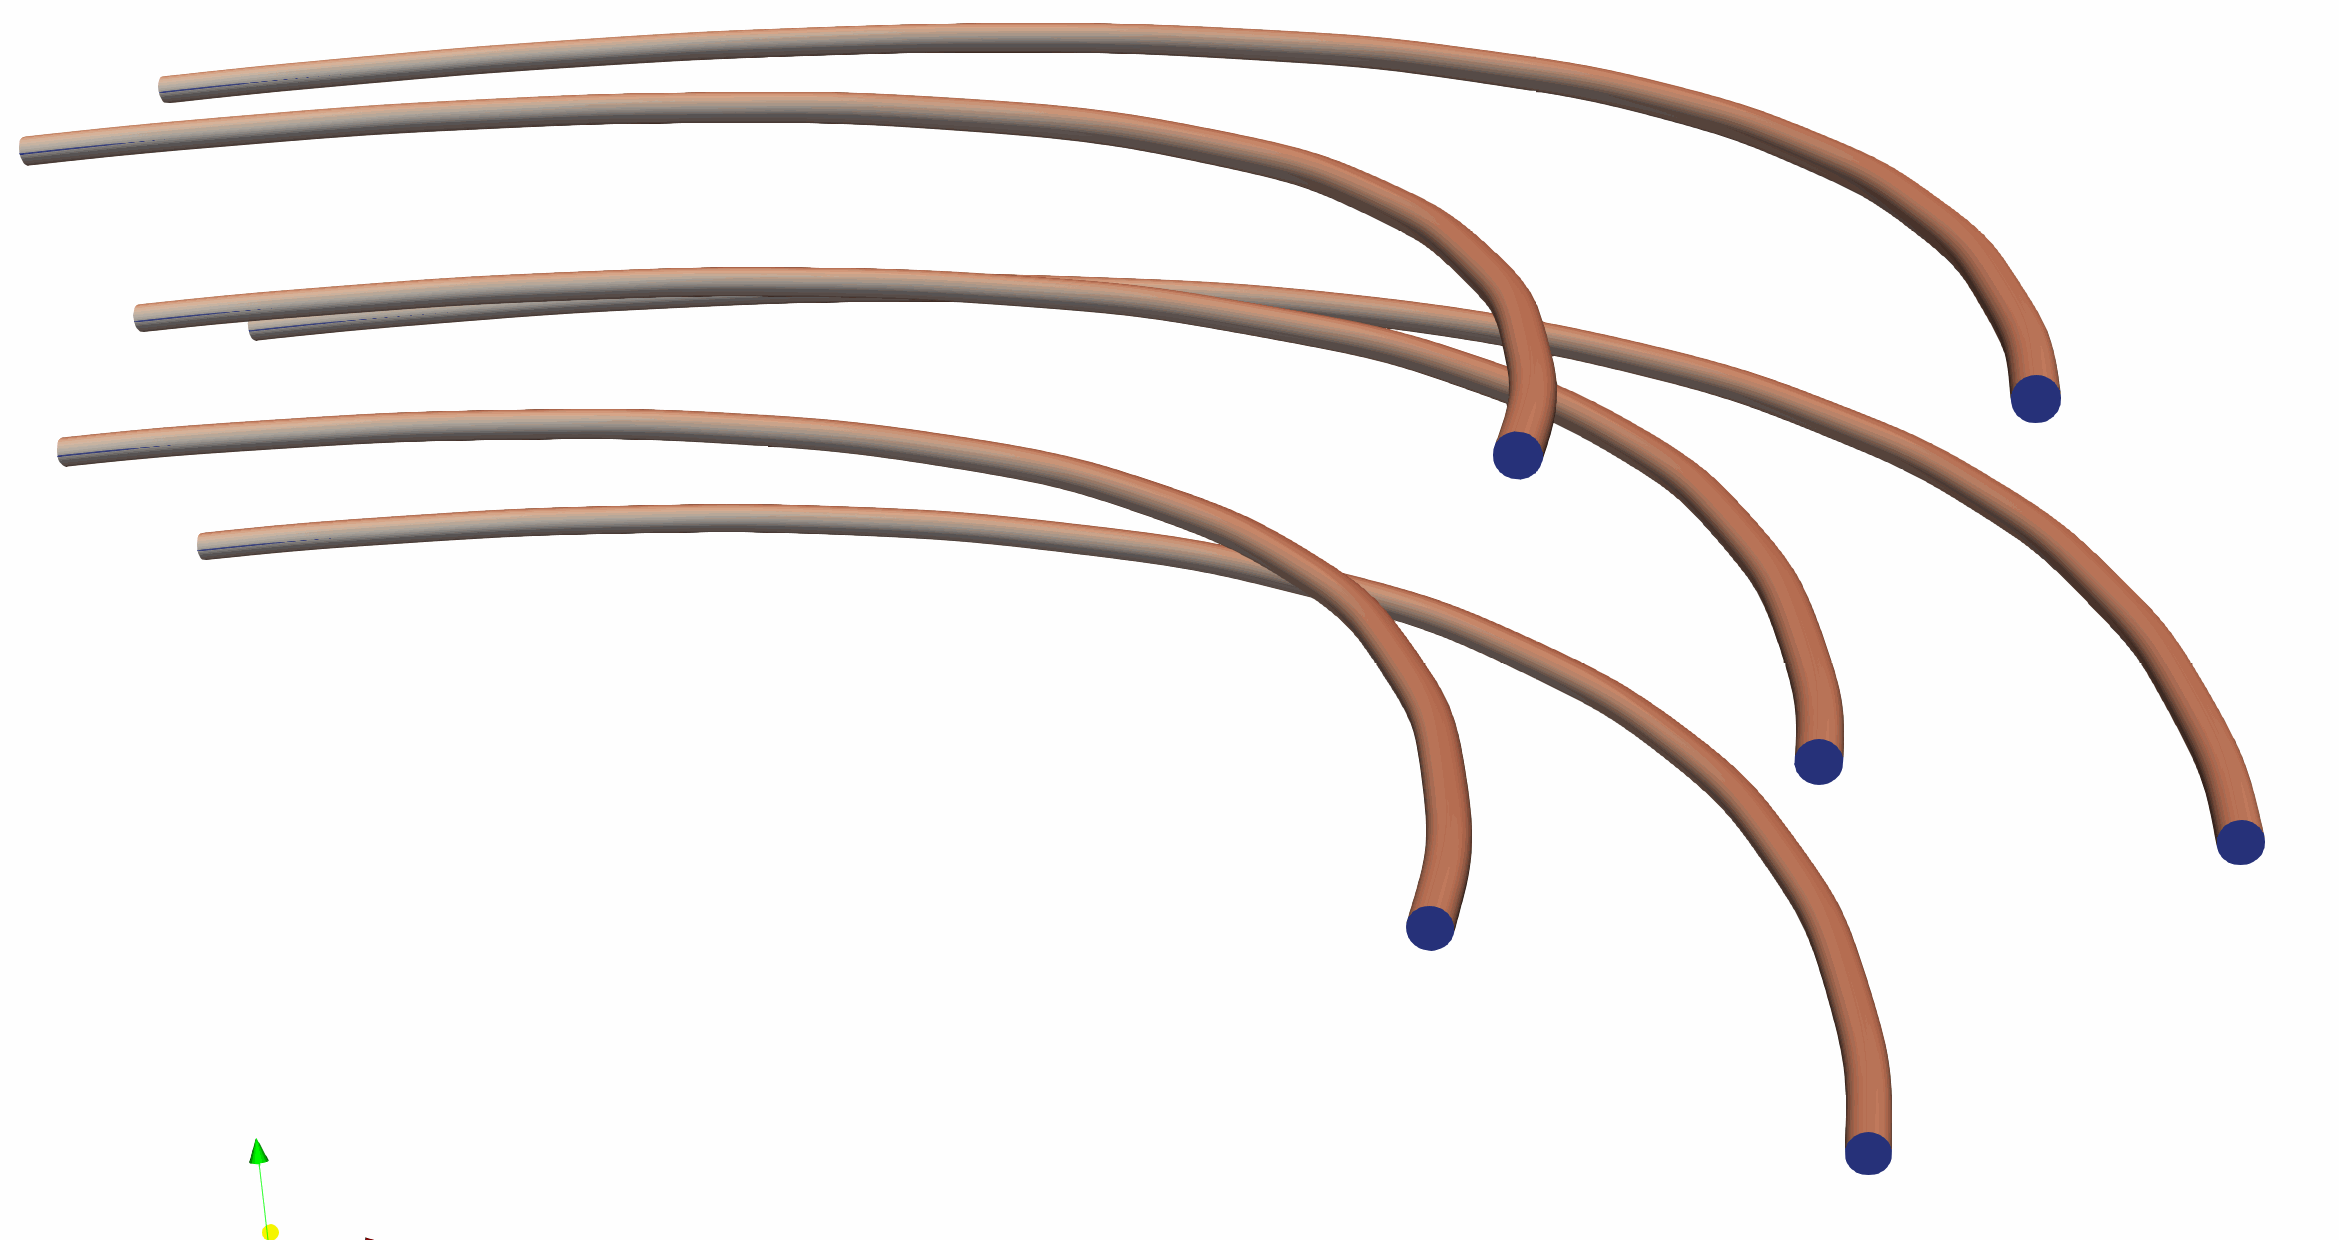
\includegraphics[scale=.05]{figures/OldAlg3D5.png}
        \caption*{(b)}
    \end{subfigure}
    \begin{subfigure}{.3\textwidth}
        \centering
        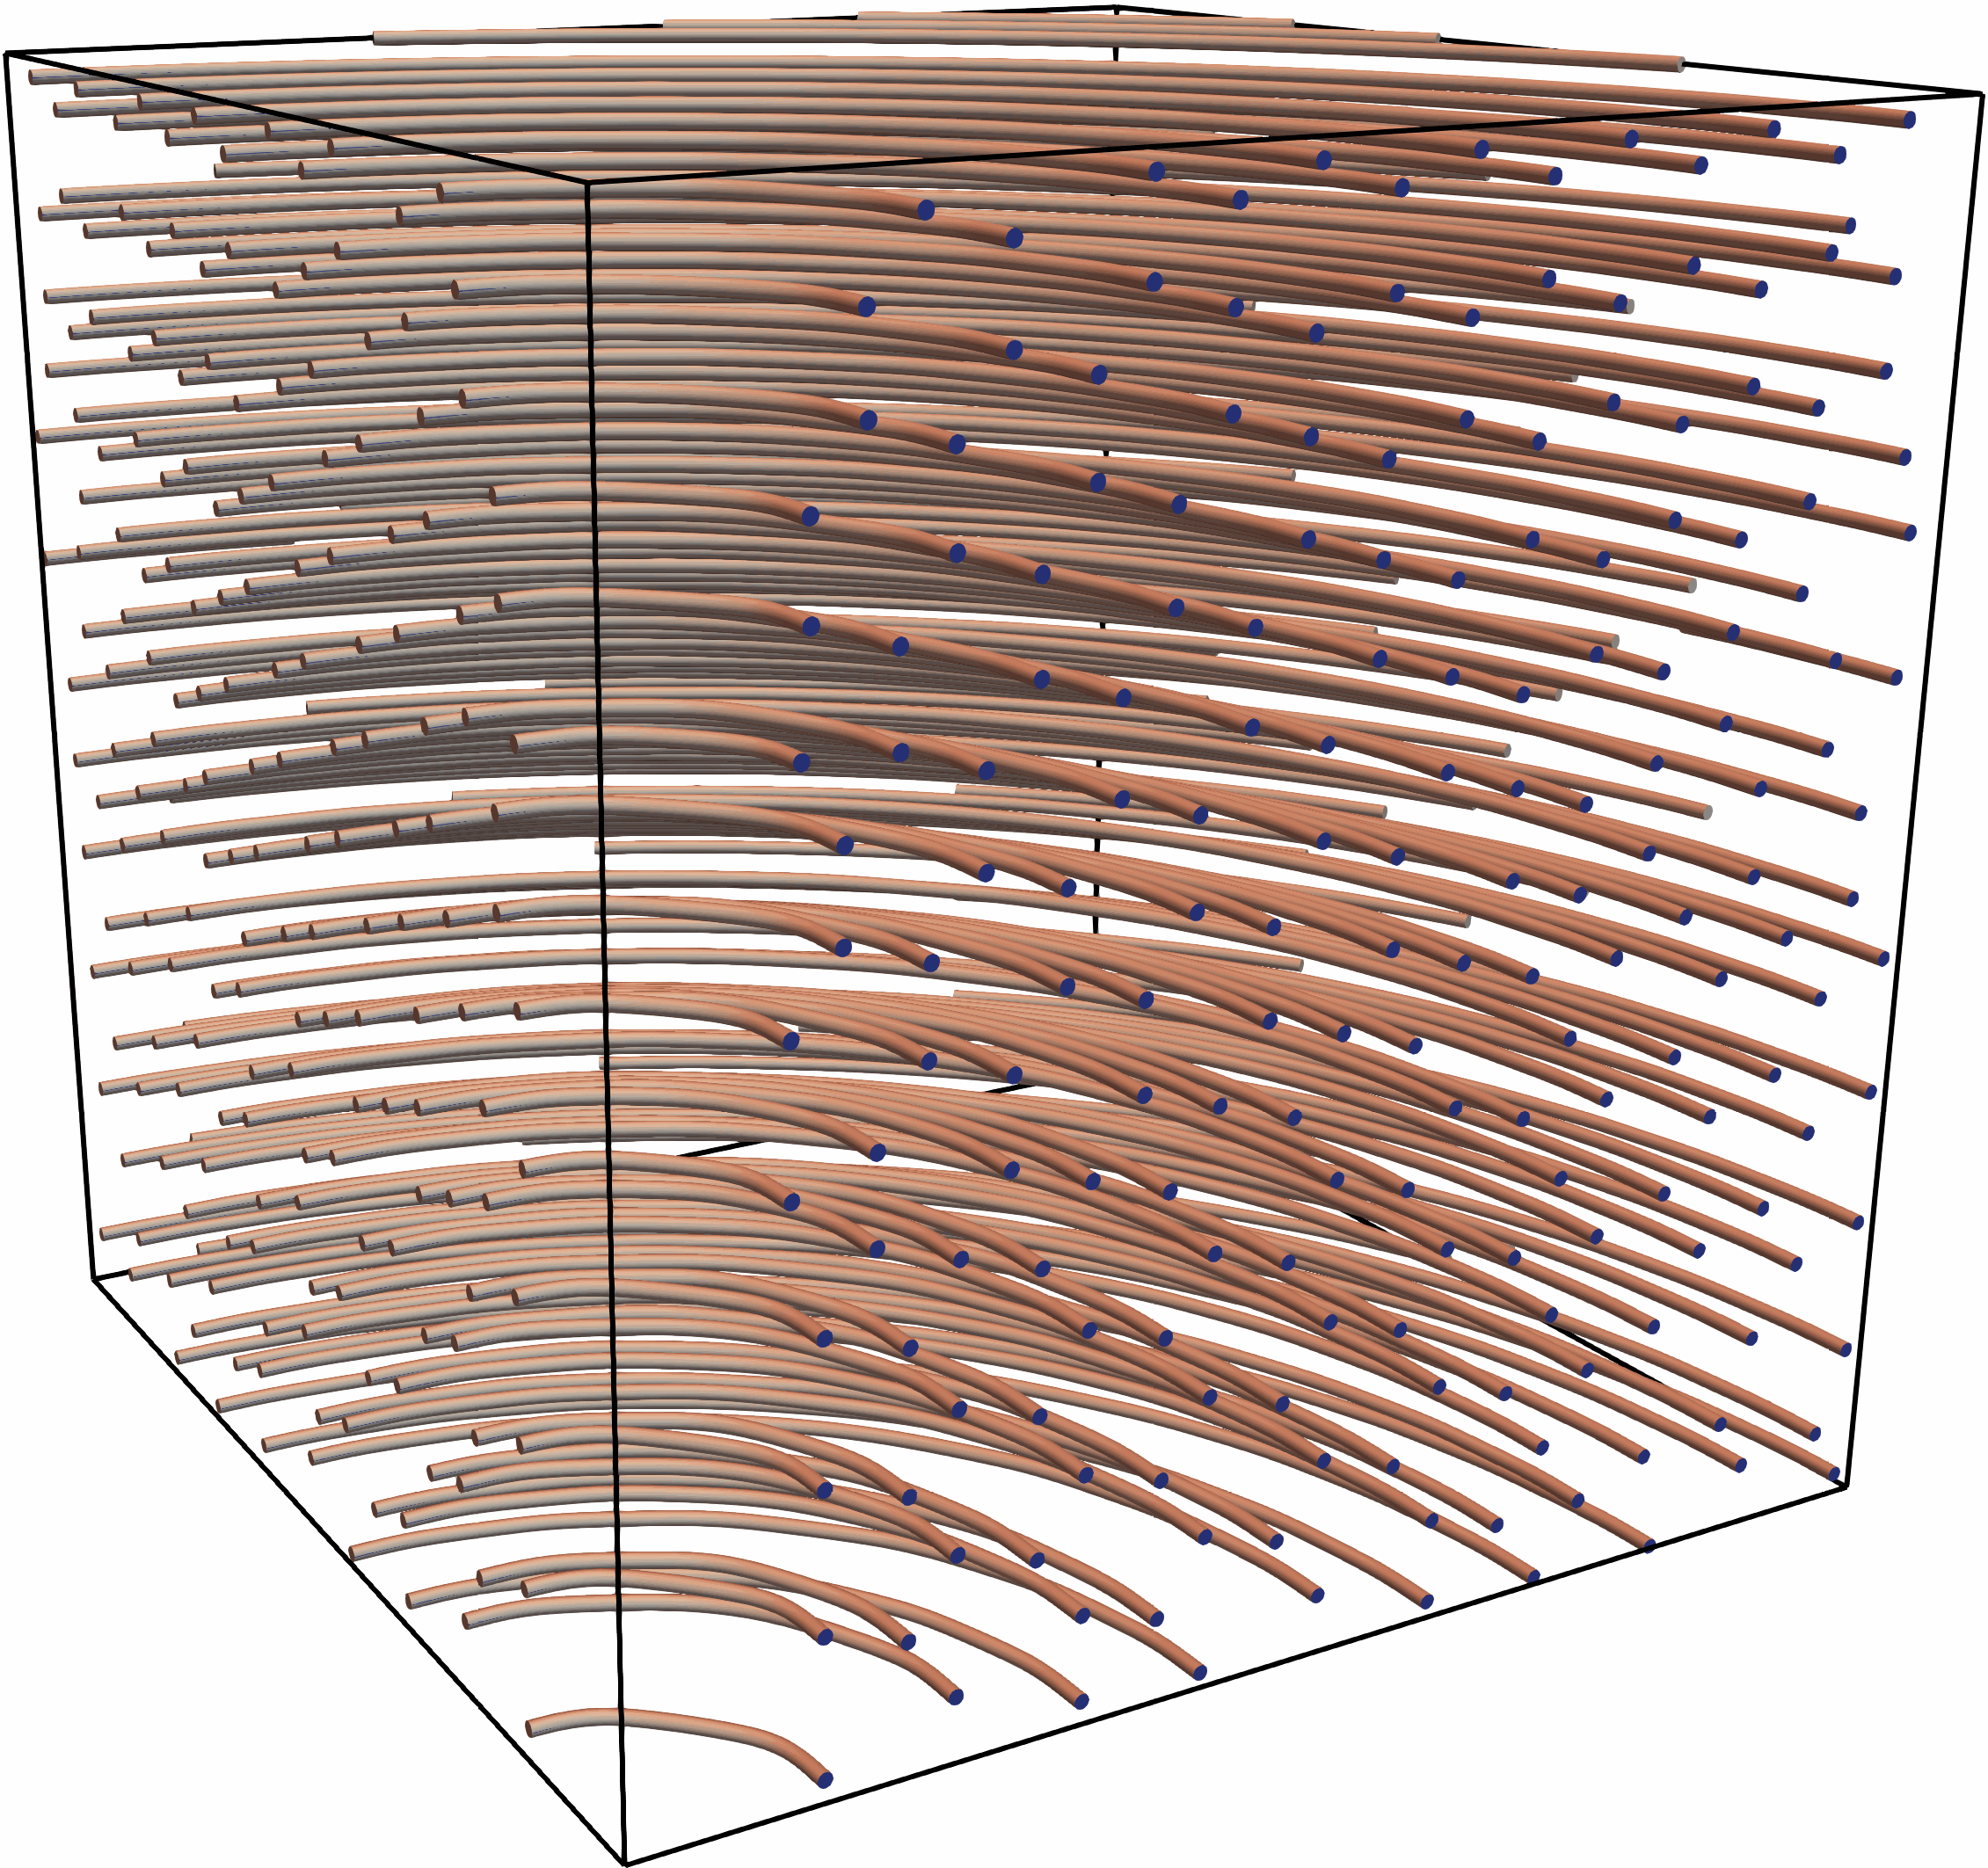
\includegraphics[scale=.05]{figures/OldAlg3D400.png}
        \caption*{(c)}
    \end{subfigure}
    \caption{
        (a): The normal plane of a streamline segment $s$ with two orthonormal basis vectors $b_0, b_1$.
        (b): A clear view of the center streamline with five neighbor streamlines evenly distributed at distance $d_S$.
        (c): A filled cube containing 254 streamlines. Notice the resemblance to \cref{fig:failedbasics} (c).
    }
    \label[figure]{fig:failed3d}
\end{figure}
The most important part to generate streamlines in 3D is obtaining the seed locations.
In three dimensions, a vector has infinitely many normals, which all lie on a plane it is a normal of.
Therefore, we define a number of points to evenly distribute around the streamline.
The process of obtaining these points is as follows.
Instead of the two trivial normals in 2D, we now construct a normal plane around the streamline trajectory at the streamline's points.
For this, we find two vectors which are linearly independent of each other and the trajectory,
and then orthonormalize them to receive two orthonormal basis vectors $b_0, b_1$ (see \cref{fig:failed3d} (a)).
Having found $b_0$ and $b_1$, we can use the roots of unity (fundamentals, \cref{rootsofunity}) to find evenly spaced points on the unit circle.
With $i$ being the complex number, we obtain $k$ roots of unity via 
\[n_j = e^{ji2\pi/k}, j = 0, 1, ..., k-1\]
Since the magnitude of $n_j$ is always one, we do a simple basis transformation into the 3D frame of reference.
We obtain the $j$-th 3D-vector $v_j$ from the $j$-th root using our basis vectors $b_0$ and $b_1$:
\[v_j = re(n_j)*b_0 + im(n_j)*b_1 \]
This gives us $k$ uniformly placed vectors in the normal plane around the current streamline segment.
The rest of the algorithm stays largely the same as in 2D, the grid used for seed filtering is extended into the 3rd dimension accordingly.
See \cref{fig:failed3d} (b, c) for an example using a 3D vector field.
\newpage
\begin{figure}[ht]
    \centering
    
\end{figure}
\subsubsection{Shortcomings}
\begin{figure}[ht]
    \begin{adjustwidth}{-2cm}{-2cm}
        \centering
        \begin{subfigure}[b]{.5\textwidth}
            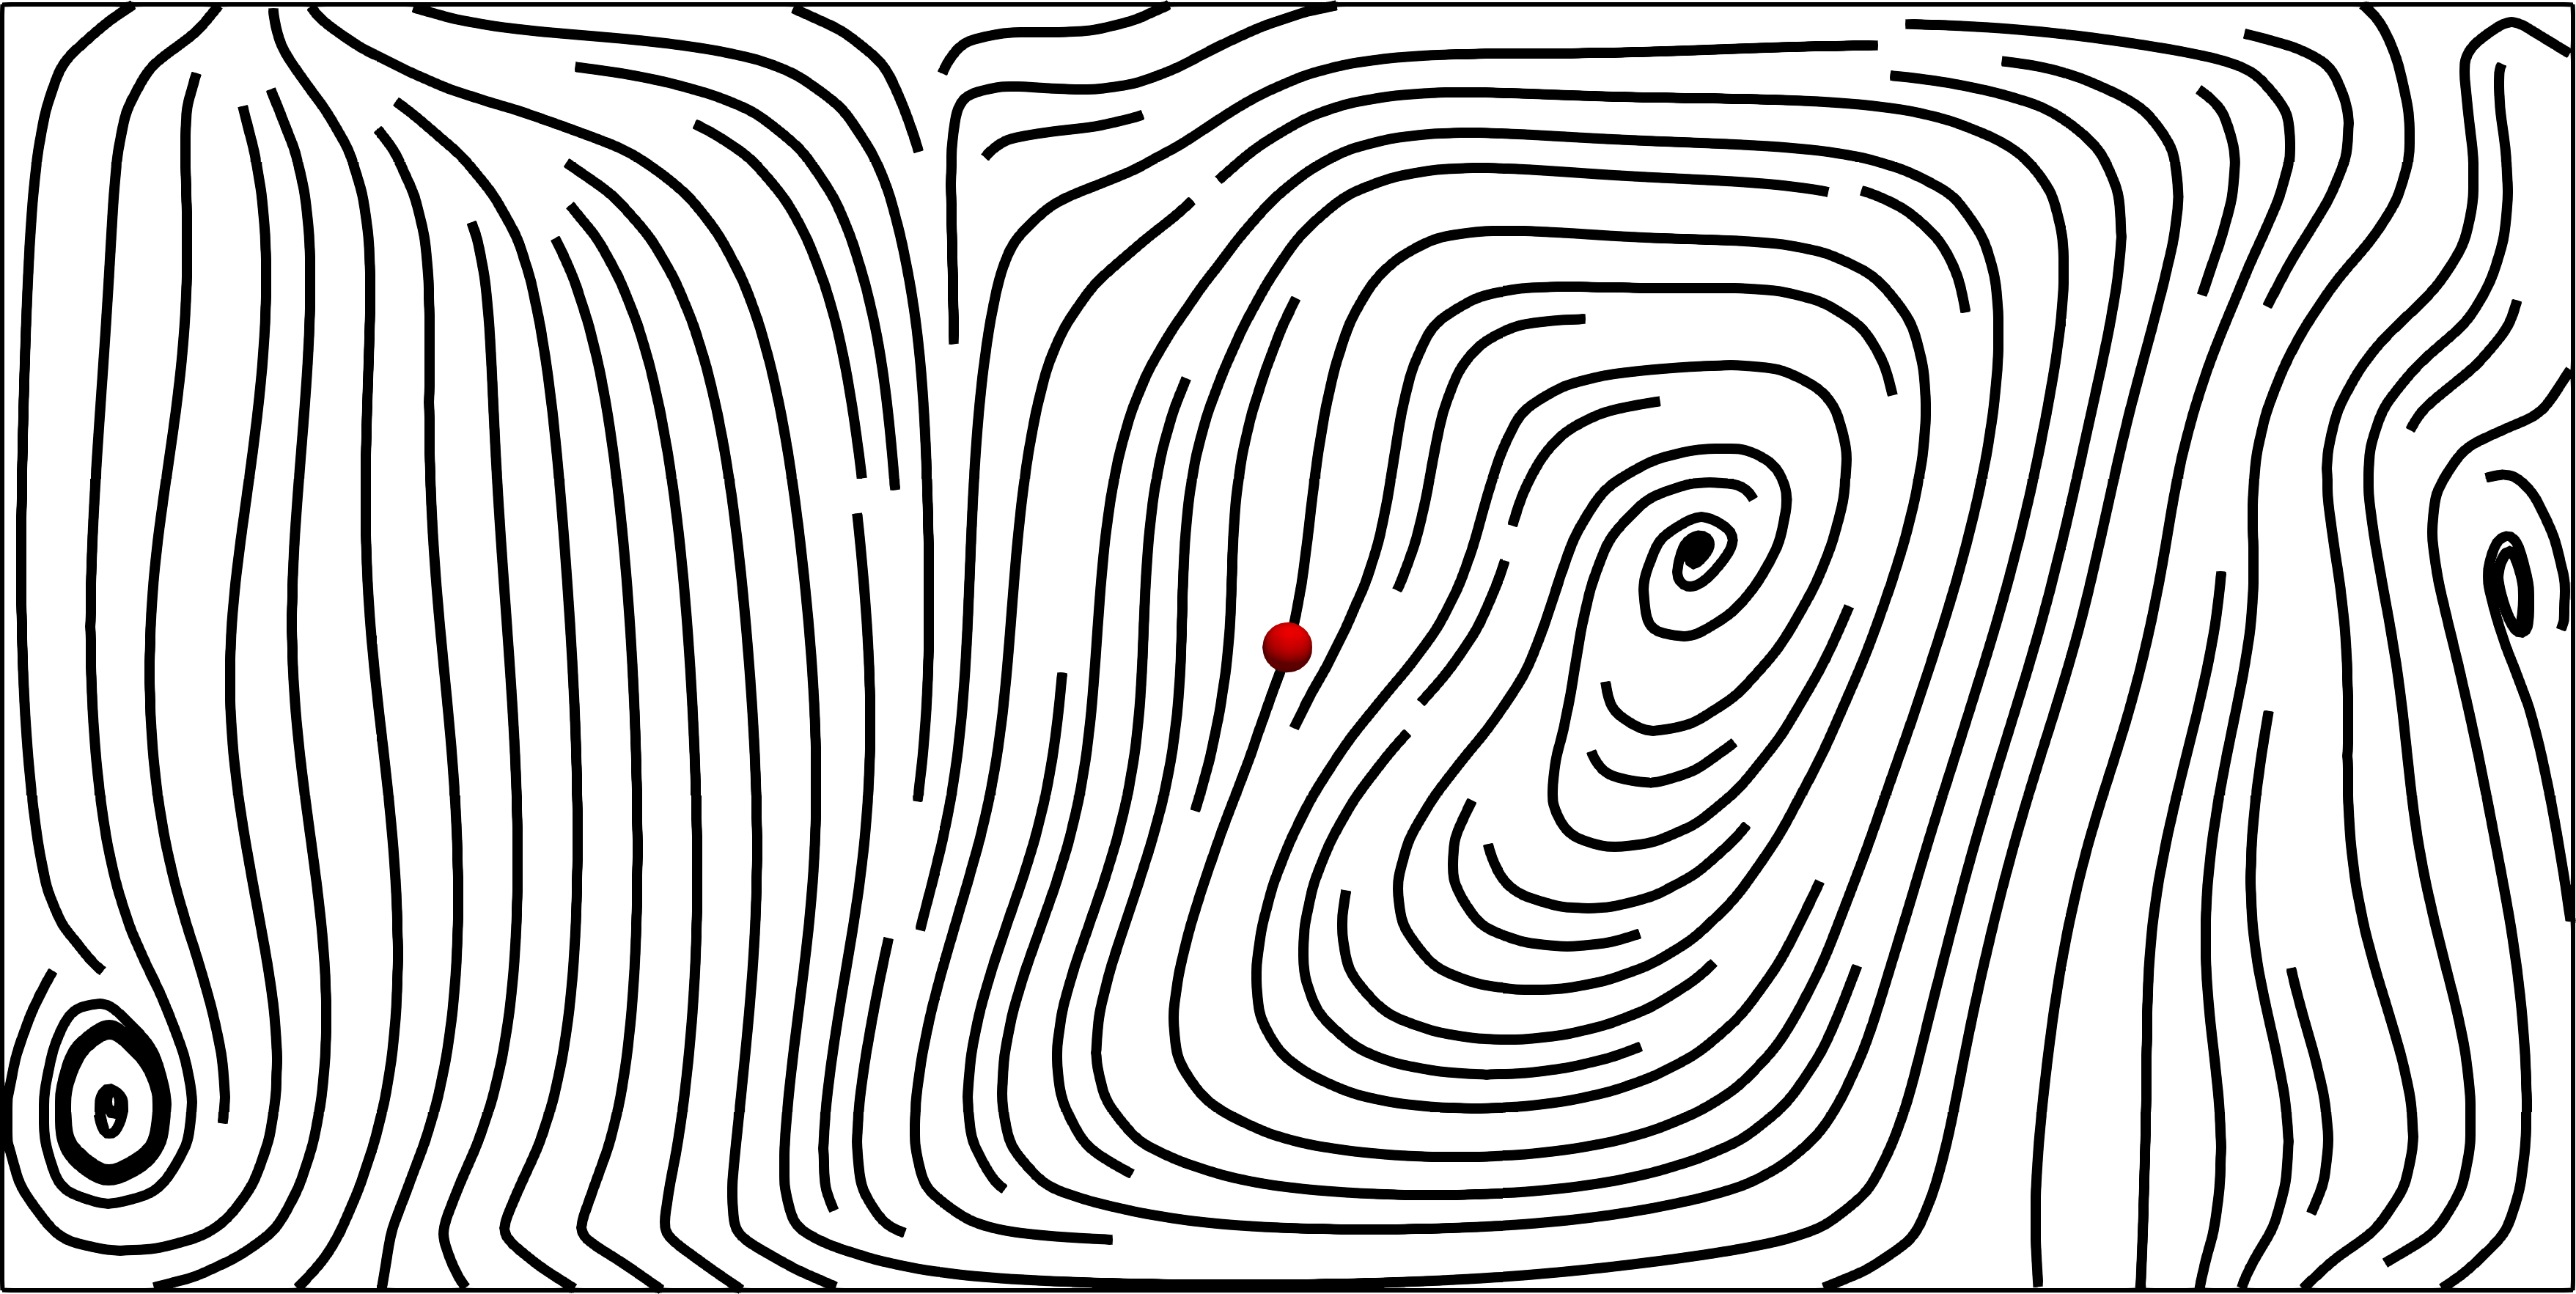
\includegraphics[scale=.075]{figures/OAH2D1.png}
            \caption*{(a)}
        \end{subfigure}
        \begin{subfigure}[b]{.5\textwidth}
            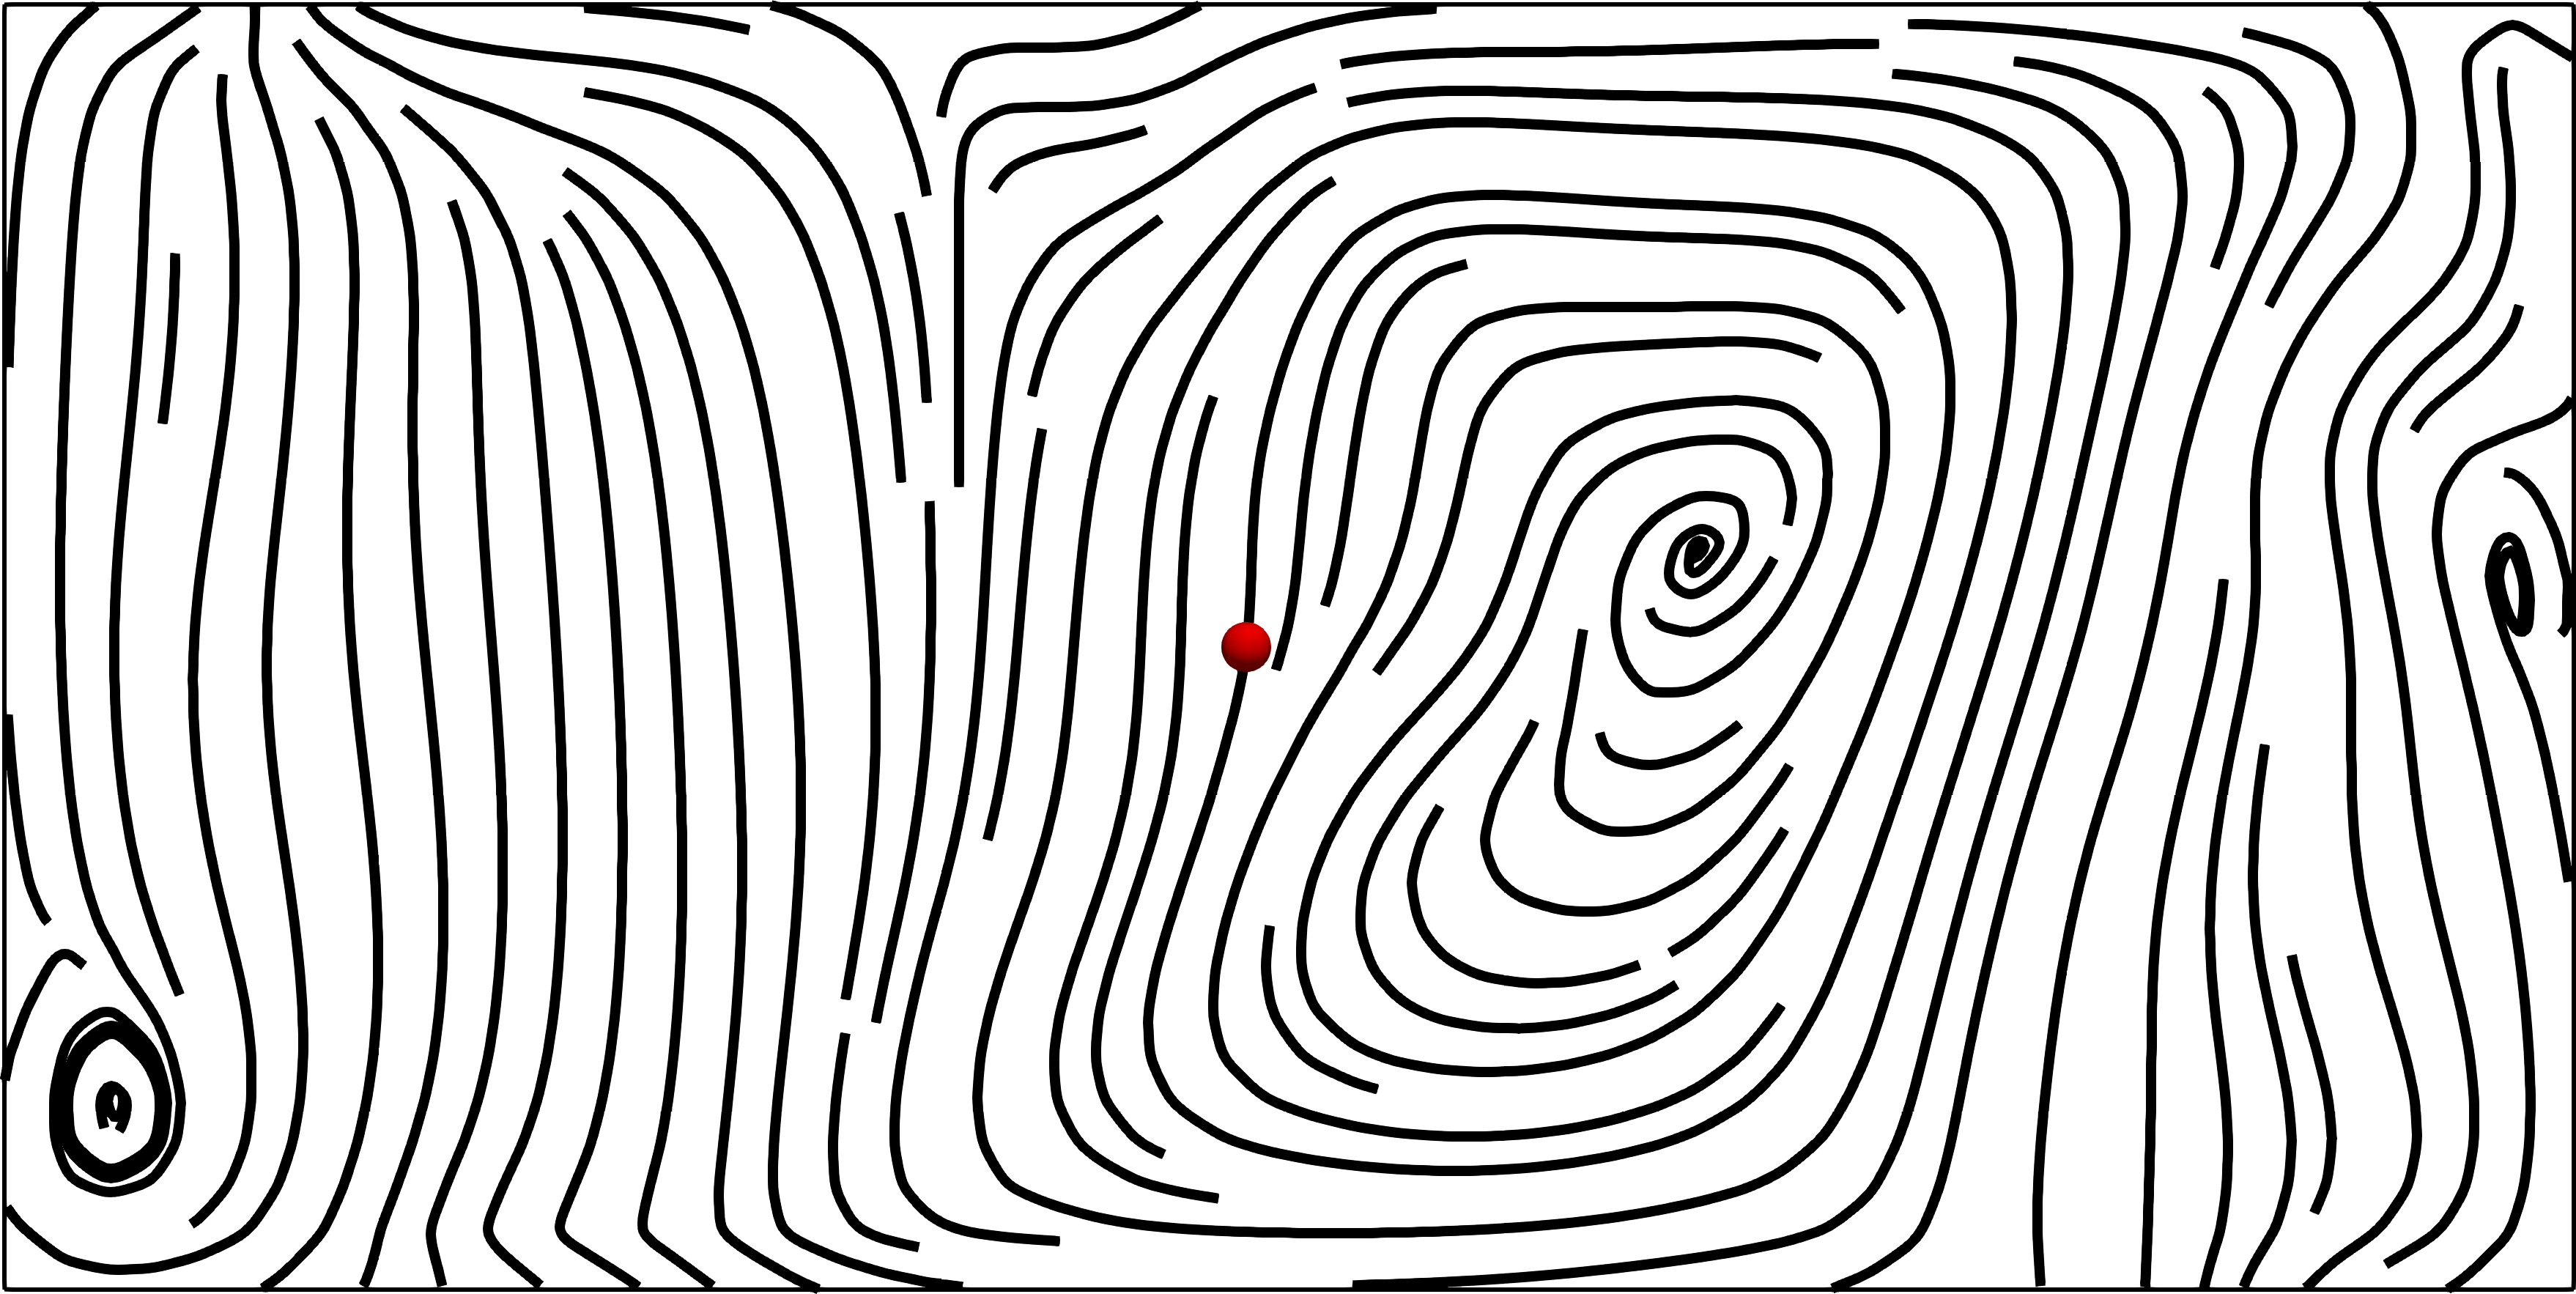
\includegraphics[scale=.075]{figures/OAH2D2.png}
            \caption*{(b)}
        \end{subfigure}
    \end{adjustwidth}
    \caption{
        Two different line placements due to a seed choice difference of only $1e-4\%$ of image width.
    }
    \label[figure]{fig:failedshift}
\end{figure}
While this algorithm can quickly fill a space with decent streamlines,
the main problem is the inability to cope with small changes to streamlines.
This is mainly a result of the strong hierarchical nature:
Since every streamline after the first comes from its predecessor,
a change at the "root" can have drastic consequences for the succeeding streamlines (see \cref{fig:failedshift}).
In the context of time coherence, this makes the algorithm unsustainable, as an unsteady field is practically guaranteed to change at least slightly in the whole domain.
To make the streamlines time coherent, we need to be able to move streamlines around without affecting the global scope too much.
With this approach, changing the position of a streamline after the generation of its neighbors causes a re-evaluation of every streamline it is a predecessor of.
Due to this problem, we do not see an effective way to implement time coherence, and supersede this algorithm in favor of an image-guided one.
\newpage
